\documentclass[12pt, a4paper]{report}
\usepackage{graphicx, array, amsthm, amssymb, amsmath, algorithm, algpseudocode, float, xcolor, thmtools, thmbox, chronology, multirow, tikz, listings}
\usepackage[english]{babel}

\makeatletter
\renewcommand\thmbox@headstyle[2]{\bfseries #1}
\makeatother
\newtheorem[style=M,bodystyle=\normalfont]{theorem}{Theorem}
\newtheorem[style=M,bodystyle=\normalfont]{corollary}{Corollary}
\newtheorem[style=M,bodystyle=\normalfont]{lemma}{Lemma}
\newtheorem[style=M,bodystyle=\normalfont]{definition}{Definition}
\newcommand{\tikzxmark}{%
\tikz[scale=0.23] {
    \draw[line width=0.7,line cap=round] (0,0) to [bend left=6] (1,1);
    \draw[line width=0.7,line cap=round] (0.2,0.95) to [bend right=3] (0.8,0.05);
}}

\definecolor{dkgreen}{rgb}{0,0.6,0}
\definecolor{gray}{rgb}{0.5,0.5,0.5}
\definecolor{mauve}{rgb}{0.58,0,0.82}
\lstset{frame=tb,
  language=Java,
  aboveskip=3mm,
  belowskip=3mm,
  showstringspaces=false,
  columns=flexible,
  basicstyle={\small\ttfamily},
  numbers=none,
  numberstyle=\tiny\color{gray},
  keywordstyle=\color{blue},
  commentstyle=\color{dkgreen},
  stringstyle=\color{mauve},
  breaklines=true,
  breakatwhitespace=true,
  tabsize=3
}


\title{Data Bases II \\ \textit{Theory}}
\author{Christian Rossi}
\date{Academic Year 2023-2024}

\begin{document}

\maketitle

\newpage

\begin{abstract}
    The course aims to prepare software designers on the effective development of database applications. 
    
    First, the course presents the fundamental features of current database architectures, with a specific emphasis on the concept of transaction and its realization in centralized 
    and distributed systems. 
    
    Then, the course illustrates the main directions in the evolution of database systems, presenting approaches that go beyond the relational model, like active databases, object 
    systems and XML data management solutions.
\end{abstract}

\newpage

\tableofcontents

\newpage

\chapter{Introduction}
    \section{Data Base Management System}
    \begin{definition}
        A \emph{Data Base Management System} is a software product capable of managing data collections that are: 
        \begin{itemize}
            \item Large: much larger than the central memory available on the computers that run the software. 
            \item Persistent: with a lifetime which is independent of single executions of the programs that access them. 
            \item Shared: used by several applications at a time. 
            \item Reliable: ensuring tolerance to hardware and software failures. 
            \item Data ownership respectful: by disciplining and controlling accesses. 
        \end{itemize}
    \end{definition}
    \begin{chronology}[5]{1990}{2020}{\textwidth}
        \event{1992}{SQL '92}
        \event{1999}{SQL '99}
        \event{2001}{Ranking in databases}
        \event{2003}{XML-related features}
        \event{2005}{NoSQL}
        \event{2006}{X-Query}
        \event{2009}{JPA final release}
        \event{2011}{Temporal databases}
        \event{2016}{JSON}
    \end{chronology}

    \section{Transactions}
    \begin{definition}
        A \emph{transaction} is an elementary, atomic unit of work performed by an application. Each transaction is conceptually encapsulated within two commands:
        \begin{itemize}
            \item Begin transaction.
            \item End transaction.
        \end{itemize}
    \end{definition}
    Within a transaction, one of the commands below is executed to signal the end of the transaction: commit or rollback. 
    \begin{definition}
        The \emph{On-Line Transaction Processing} (OLTP) is a system that supports the execution of transactions on behalf of concurrent applications. 
    \end{definition}
    The application can run many transactions. So, the transactions are part of the application and not vice-versa. The transactions follow the ACID property: 
    \begin{enumerate}
        \item Atomicity: a transaction is an indivisible unit of execution. This means that all the operations in the transaction are executed or none is executed. The time in which 
            commit is executed marks the instant in which the transaction ends successfully: an error before should cause the rollback and an error after should not alter the 
            transaction. The rollback of the work performed can be caused by a rollback statement or by the DBMS. In case of a rollback, the work performed must be undone, bringing 
            the database to the state it had before the start of the transaction. It is the application's responsibility to decide whether an aborted transaction must be redone or not. 
        \item Consistency: A transaction must satisfy the database integrity constraints, that is if the initial state $S_0$ is consistent then the final state $S_f$ is also 
            consistent. This is not necessarily true for the intermediate states $S_i$. 
        \item Isolation: the execution of a transaction must be independent of the concurrent execution of other transactions. 
        \item Durability: the effect of a transaction that has successfully committed will last forever, independently of any system fault. 
    \end{enumerate}
    \begin{table}[H]
        \centering
        \begin{tabular}{c|c|c}
        \textbf{Property} & \textbf{Actions}       & \textbf{Architectural element} \\ \hline
        Atomicity         & Abort-rollback-restart & Query Manager                  \\
        Consistency       & Integrity checking     & Integrity Control System       \\
        Isolation         & Concurrency control    & Concurrency Control System     \\
        Durability        & Recovery management    & Reliability Manager           
        \end{tabular}
    \end{table}
    \begin{figure}[H]
        \centering
        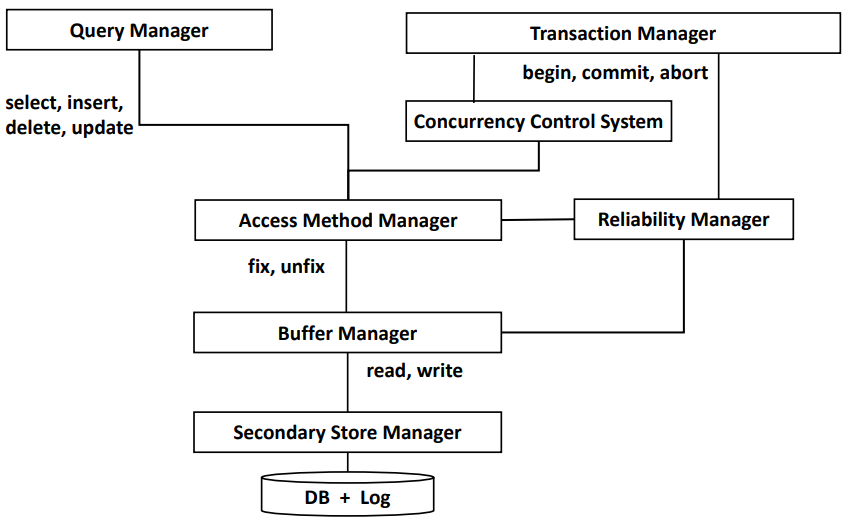
\includegraphics[width=0.75\linewidth]{images/architecture.png}
        \caption{Architecture of a Data Base Management System}
    \end{figure}

\newpage

\chapter{Concurrency}
    \section{Introduction}
    A DBMS usually needs to manage multiple applications. A unit of measurement used to evaluate the DBMS workload is the number of transaction per second ($tps$) handled by it. 
    To have an efficient usage of the database the DBMS needs to be able to handle concurrency while avoiding the insurgence of anomalies. 
    The concurrency control system schedules the order of the various transactions. 
    
    \section{Anomalies in concurrent transactions}
    The anomalies caused by uncorrect scheduling are: 
    \begin{itemize}
        \item Lost update: an update is applied from a state that ignores a preceding update, which is lost.
            \begin{table}[H]
                \centering
                \begin{tabular}{c|c}
                \textbf{Transaction $t_1$}    & \textbf{Transaction $t_2$} \\ \hline
                $r_1(x)$                      &                            \\
                $x=x+1$                       &                            \\
                                              & $r_2(x)$                   \\
                                              & $x=x+1$                    \\
                                              & $w_2(x)$                   \\
                                              & commit                     \\
                $w_1(x)$                      &                            \\
                commit                        &                           
                \end{tabular}
            \end{table}
        \item Dirty read: an uncommitted value is used to update the data. 
            \begin{table}[H]
                \centering
                \begin{tabular}{c|c}
                \textbf{Transaction $t_1$} & \textbf{Transaction $t_2$} \\ \hline
                $r_1(x)$                   &                            \\
                $x=x+1$                    &                            \\
                $w_1(x)$                   &                            \\
                                        & $r_2(x)$                   \\
                                        & commit                     \\
                abort                      &                           
                \end{tabular}
            \end{table}
        \item Non-repeatable read: someone else updates a previously read value.
            \begin{table}[H]
                \centering
                \begin{tabular}{c|c}
                \textbf{Transaction $t_1$}  & \textbf{Transaction $t_2$} \\ \hline
                $r_1(x)$                    &                            \\
                                            & $r_2(x)$                   \\
                                            & $x=x+1$                    \\
                                            & $w_2(x)$                   \\
                                            & commit                     \\
                $r_1(x)$                    &                            \\
                commit                      & \multicolumn{1}{l}{}      
                \end{tabular}
            \end{table}
        \item Phantom update: someone else updates data that contributes to a previously valid constraint. 
            \begin{table}[H]
                \centering
                \begin{tabular}{c|c}
                \textbf{Transaction $t_1$} & \textbf{Transaction $t_2$} \\ \hline
                $r_1(x)$                   &                            \\
                                           & $r_2(y)$                   \\
                $r_1(y)$                   &                            \\
                                           & $y=y-100$                  \\
                                           & $r_2(z)$                   \\
                                           & $z=z+100$                  \\
                                           & $w_2(y)$                   \\
                                           & $w_2(z)$                   \\
                                           & commit                     \\
                $r_1(z)$                   &                            \\
                $s=x+y+z$                  &                            \\
                commit                     &                           
                \end{tabular}
            \end{table}
        \item Phantom insert: someone else inserts data that contributes to a previously read datum.
    \end{itemize}

    \section{Concurrency theory}
    \begin{definition}
        A \emph{model} is an abstraction of a system, object or process, which purposely disregards details to simplify the investigation of relevant properties. 
    \end{definition}
    Concurrency theory builds upon a model of transaction and concurrency control principles that help understanding the real systems. Real systems exploit implementation level 
    mechanisms which help achieve some desirable properties postulated by the theory. 
    \begin{definition}
        An \emph{operation} consist in a reading or in a writing of a specific datum by a specific transaction. 

        A \emph{schedule} is a sequence of operations performed by concurrent transactions that respects the order of operations of each transaction. 
    \end{definition}
    The transactions can be: serial, interleaved or nested. The number of serial schedules for $n$ transaction is equal to: 
    \[N_S=n!\]
    While the total number of distinct schedules given the number of transaction $n$ is equal to: 
    \[N_D=\dfrac{\left( \sum_{i=1}^nk_i \right)!}{\prod_{i=1}^n \left( k_i! \right)}\]
    \begin{example}
        Given two transaction $T_1$ and $T_2$ we have six possible different schedules, where only two are serial:
        \begin{enumerate}
            \item $r_1(x) w_1(x) r_2(z) w2(z)$
            \item $r_2(z) w_2(z) r_1(x) w_1(x)$
            \item $r_1(x) r_2(z) w_1(x) w_2(z)$
            \item $r_2(z) r_1(x) w_2(z) w_1(x)$
            \item $r_1(x) r_2(z) w_2(z) w_1(x)$
            \item $r_2(z) r_1(x) w_1(x) w_2(z)$
        \end{enumerate}
        The first two are serial, the third and the fourth are nested, and the last two interleaved.
    \end{example}
    The concurrency control has to reject all the schedules that causes anomalies. 
    \begin{definition}
        The \emph{scheduler} is a component that accepts or rejects operations requested by the transactions. 

        The \emph{serial schedule} is a schedule in which the actions of each transaction occur in a contiguous sequence.
    \end{definition}
    A serializable schedule leaves the database in the same state as some serial schedule of the same transactions, so it is correct. To introduce other classes we have to initially
    make two assumptions: 
    \begin{itemize}
        \item The transactions are observed a posteriori. 
        \item Commit-projection: consider only the committed transactions. 
    \end{itemize}

    \section{View-serializability}
    \begin{definition}
        $r_i(x)$ \emph{reads-from} $w_j(x)$ when  $w_j(x)$  precedes  $r_i(x)$ and there is no  $w_k(x)$ in $S$ between  $r_i(x)$  and  $w_j(x)$. 
        
        $w_i(x)$ in a schedule $S$ is a \emph{final write} if it is the last write on $x$ that occurs in $S$. 


        Two schedules are said to be \emph{view-equivalent} ($S_i \approx_V S_j$) if they have:
        \begin{enumerate}
            \item The same operations. 
            \item The same reads-from relationships.
            \item The same final writes. 
        \end{enumerate}
    \end{definition}

    A schedule is view-serializable (VSR) if it is view-equivalent to a serial schedule of the same transactions. The value written by $w_j(x)$ could be uncommitted when $r_i(x)$ 
    reads it, but we are sure that it will be committed (commit-projection hypotesis).
    \begin{example}
        The following schedules are given:
        \begin{itemize}
            \item $S_1: w_0(x) r_2(x) r_1(x) w_2(x) w_2(z)$
            \item $S_2: w_0(x) r_1(x) r_2(x) w_2(x) w_2(z)$
            \item $S_3: w_0(x) r_1(x) w_1(x) r_2(x) w_1(z)$
            \item $S_4: w_0(x) r_1(x) w_1(x) w_1(z) r_2(x)$
            \item $S_5: r_1(x) r_2(x) w_1(x) w_2(x)$
            \item $S_6: r_1(x) r_2(x) w_2(x) r_1(x)$
            \item $S_7: r_1(x) r_1(y) r_2(z) r_2(y) w_2(y) w_2(z) r_1(z)$
        \end{itemize}
        We have that only $S_2$ and $S_3$ are serial. $S_1$ is view-equivalent to serial schedule $S_2$ (so it is view-serializable). 
        $S_3$ is not view-equivalent to $S_2$ (different operations) but is view-equivalent to serial schedule $S_4$, so it is also view-serializable. 

        $S_5$ corresponds to a lost update, $S_6$ corresponds to a non-repeatable read, and $S_7$ corresponds to a phantom update. All these schedules are non view-serializable. 
        
        The following schedules are given:
        \begin{itemize}
            \item $S_a: w_0(x) r_1(x) w_0(z) r_1(z) r_2(x) w_0(y) r_3(z) w_3(z) w_2(y) w_1(x) w_3(y)$
            \item $S_b: w_0(x) w_0(z) w_0(y) r_2(x) w_2(y) r_1(x) r_1(z) w_1(x) r_3(z) w_3(z) w_3(y)$
            \item $S_c: w_0(x) w_0(z) w_0(y) r_2(x) w_2(y) r_3(z) w_3(z) w_3(y) r_1(x) r_1(z) w_1(x)$
        \end{itemize}
        $S_a$ and $S_b$ are view-equivalent because all the reads-from relationship and final writes are the same. In fact, we have: 
        \begin{itemize}
            \item Reads-from: $r_1(x)$ from $w_0(x)$, $r_1(z)$ from $w_0(z)$, $r_2(x)$ from $w_0(x)$, $r_3(z)$ from $w_0(z)$.
            \item Final writes: $w_1(x)$, $w_3(y)$, $w_3(z)$.
        \end{itemize}
        $S_a$ and $S_c$ are not view-equivalent because not all the reads-from relationship are the same. 
    \end{example}
    Deciding if a generic schedule is in VSR is a NP-complete problem. Therefore, we need to find a stricter definition that is easier to check. The new definition may lead to 
    rejecting some schedule that would be acceptable under view-serializability but not under the stricter criterion.
    
    \section{Conflict-serializability}
    \begin{definition}
        Two operations $o_i$ and $o_j$ ($i \neq j$) are in \emph{conflict} if they address the same resource and at least one of them is write. There are two possible cases:
        \begin{enumerate}
            \item Read-write conflicts ($r-w$ or $w-r$).
            \item Write-write conflicts ($w-w$).
        \end{enumerate}

        Two schedules are \emph{conflict-equivalent} ($S_i \approx_C S_j$) if $S_i$ and $S_j$ contain the same operations and in all the conflicting pairs the transactions occur 
        in the same order. 

        A schedule is \emph{conflict-serializable} (CSR) if and only if it is conflict equivalent to a serial schedule of the same transactions. 
    \end{definition}
    We have that VSR is a strict subset of CSR and that CSR implies VSR. 
    \begin{proof}[VSR is a subset of CSR]
        Schedule $S = r_1(x) w_2(x) w_1(x) w_3(x)$ is: 
        \begin{itemize}
            \item View-serializable.
            \item Not conflict-serializable
        \end{itemize}
        It is possible to check that there is no conflict-equivalent serial schedule.
    \end{proof}
    \begin{proof}[CSR implies VSR]
        We assume $S_1 \approx_C S_2$ and prove that $S_1 \approx_V S_2$. $S_1$ and $S_2$ must have: 
        \begin{itemize}
            \item The same final writes: if they didn't, there would be at least two writes in a different order, and since two
                writes are conflicting operations, the schedules would not be $\approx_C$. 
            \item The same reads-from relations: if not, there would be at least one pair of conflicting operations in a different
                order, and therefore, again, $\approx_C$ would be violated. 
        \end{itemize}
    \end{proof}
    The testing of view-serializability is done with a conflict graph that has one node for each transaction $T_i$, and one arc from $T_i$ to $T_j$ if there exists at least one conflict between an operation $o_i$ of $T_i$ and an operation $o_j$ of $T_j$ such that $o_i$ precedes $o_j$.
    \begin{theorem}
        A schedule is \emph{conflict-serializable} if and only if its conflict graph is acyclic.
    \end{theorem}
    \begin{example}
        We are given the schedule \[S: w_0(x) r_1(x) w_0(z) r_1(z) r_2(x) w_0(y) r_3(z) w_3(z) w_2(y) w_1(x) w_3(y)\]
        To test the conflict serializability we have to do the following steps: 
        \begin{enumerate}
            \item Create all the nodes based on the number of transactions of the schedule. 
            \item Divide the operation based on resource requested.
            \item Check all the write-write and read-write relationships in each subset, and add the arcs based on these. 
        \end{enumerate}
        In the given example we obtain: 
        \begin{itemize}
            \item $x: w_0 r_1 r_2 w_1$
            \item $y: w_0 w_2 w_3$
            \item $z: w_0 r_1 r_3 w_3$
        \end{itemize}
        \begin{figure}[H]
            \centering
            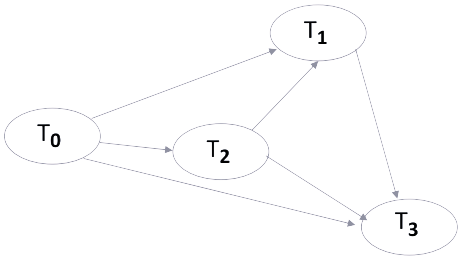
\includegraphics[width=0.5\linewidth]{images/conflict.png}
        \end{figure}
        There are no cycles in the graph, so this means that the schedule is CSR. 
    \end{example}
    \begin{proof}[CSR implies acyclicity of the conflict graph]
        Consider a schedule $S$ in $CSR$. As such, it is $\approx_C$ to a serial schedule. 
        Without loss of generality we can label the transactions of $S$ to say that their order in the serial schedule is: $T_1 T_2 \dots T_n$.
        Since the serial schedule has all conflicting pairs in the same order as schedule $S$, in the conflict graph there can only be arcs $(i,j)$, with $i<j$. 
        Then the graph is acyclic, as a cycle requires at least an arc $(i,j)$ with $i>j$.
    \end{proof}
    \begin{proof}[acyclicity of the conflict graph implies CSR]
        If $S$'s graph is acyclic then it induces a topological (partial) ordering on its nodes. The same partial order exists on the transactions of $S$. 
        Any serial schedule whose transactions are ordered according to the partial order is conflict-equivalent to $S$, because for all conflicting pairs $(i,j)$ it is always $i<j$. 
    \end{proof}
        
    \section{Concurrency control in practice}
    Conflict-serializability checking would be efficient if we knew the graph from the beginning, but usually we don't. Therefore, a scheduler must rather work online. 
    So, it is not feasible to maintain the conflict graph, update it, and check its acyclicity at each operation request. At the same time, the assumption that concurrency control 
    can work only with the commit-projection of the schedule is unrealistic because aborts do occur. We need some simple online decision criterion for the scheduler, which must 
    avoid as many anomalies as possible, and have negligible overhead. 
        
    When dealing with online concurrency control, it is important also to consider arrival sequences. The concurrency control system maps an arrival sequence into an effective a 
    posteriori schedule. To implement this online scheduling we use two main families of techniques:
    \begin{itemize}
        \item Pessimistic (locks): if a resource is taken, make the requester wait or pre-empt the holder.
        \item Optimistic (timestamps and versions): serve as many requests as possible, possibly using out-of-date versions of the data. 
    \end{itemize}
    Usually, commercial systems take the best of both worlds. 

    \section{Locking}
    The method called locking is the most used in commercial systems. A transaction is well-formed with respect to locking if: 
    \begin{itemize}
        \item Read operations are preceded by $r\_lock$ (shared) and followed by unlock. 
        \item Write operations are preceded by $w\_lock$ (exclusive) and followed by unlock. 
    \end{itemize}
    In both cases unlocking can be delayed with respect to the end of the operations. So, every object can be: free, r-locked or w-locked. 

    Transactions that first read and then write an object may acquire a $w\_lock$ already when reading or acquire a $r\_lock$ first and then upgrade it into a $w\_lock$ (escalation).

    The lock manager receives requests from the transactions and grants resources according to the conflict table: 

    \begin{table}[H]
        \centering
        \begin{tabular}{cccc}
        \textbf{}                              & \multicolumn{3}{c}{\textbf{Resource status}}                                                                                                                                                                                                   \\ \cline{2-4} 
        \multicolumn{1}{c|}{\textbf{Request}}  & \multicolumn{1}{c|}{\textit{FREE}}                                          & \multicolumn{1}{c|}{\textit{R\_LOCKED}}                                            & \multicolumn{1}{c|}{\textit{W\_LOCKED}}                                     \\ \hline
        \multicolumn{1}{|c|}{\textit{r\_lock}} & \multicolumn{1}{c|}{\begin{tabular}[c]{@{}c@{}}\checkmark\\ R\_LOCKED\end{tabular}} & \multicolumn{1}{c|}{\begin{tabular}[c]{@{}c@{}}\checkmark\\ R\_LOCKED($n++$)\end{tabular}} & \multicolumn{1}{c|}{\begin{tabular}[c]{@{}c@{}}\tikzxmark\\ W\_LOCKED\end{tabular}} \\ \hline
        \multicolumn{1}{|c|}{\textit{w\_lock}} & \multicolumn{1}{c|}{\begin{tabular}[c]{@{}c@{}}\checkmark\\ W\_LOCKED\end{tabular}} & \multicolumn{1}{c|}{\begin{tabular}[c]{@{}c@{}}\tikzxmark\\ R\_LOCKED\end{tabular}}        & \multicolumn{1}{c|}{\begin{tabular}[c]{@{}c@{}}\tikzxmark\\ W\_LOCKED\end{tabular}} \\ \hline
        \multicolumn{1}{|c|}{\textit{unlock}}  & \multicolumn{1}{c|}{ERROR}                                                  & \multicolumn{1}{c|}{\begin{tabular}[c]{@{}c@{}}\checkmark\\ $n--$\end{tabular}}            & \multicolumn{1}{c|}{\begin{tabular}[c]{@{}c@{}}\checkmark\\ FREE\end{tabular}}      \\ \hline
        \end{tabular}
    \end{table}

    \begin{example}
        Given a schedule with three transactions and the following operations: 
        \[r_1(x)w_1(x)r_2(x)r_3(y)w_1(y)\]
        We have the following locks: 
        \begin{itemize}
            \item $r_1(x)$: $r_1\_lock(x)$ request $\rightarrow$ Ok $\rightarrow$ $x$ is $r-locked$ with $n_x=1$. 
            \item $w_1(x)$: $w_1\_lock(x)$ request $\rightarrow$ Ok $\rightarrow$ $x$ is $w-locked$. 
            \item $r_2(x)$: $r_1\_lock(x)$ request $\rightarrow$ No, because $x$ is $w-locked$ $\rightarrow$ $T_2$ waits. 
            \item $r_3(y)$: $r_3\_lock(y)$ request $\rightarrow$ Ok $\rightarrow$ $y$ is $r-locked$ with $n_y=1$ and then $T_3$ unlocks $y$. 
            \item $w_1(y)$: $w_1\_lock(y)$ request $\rightarrow$ Ok $\rightarrow$ $y$ is $w-locked$ and then $x$ and $y$ are freed. 
        \end{itemize}
        So, the schedule a posteriori will become: 
        \[r_1(x)w_1(x)r_3(y)w_1(y)r_2(x)\]
        and we have that the transaction two is delayed. 
    \end{example}
    The locking system is implemented via lock tables, which are hash tables indexing the lockable items via hashing and where each locked item has a linked list associated with it. 
    Every node in the linked list represents the transaction which requested for lock, the lock mode and the current status. Every new lock request for the data item is appended to 
    the list.

    \section{Two-phase locking}
    With the locking showed before we do not eliminate the anomalies caused by non-repeatable reads. To avoid this problem we can use a two-phase rule which requires that a 
    transaction cannot acquire any other lock after releasing one. So, we have a phase where the transaction acquires all the locks, a phase where it executes all operations and 
    a final phase of unlocking. 
    \begin{definition}
        The class of \emph{two-phase locking} is the set of all schedules generated by a scheduler that: 
        \begin{itemize}
            \item Only processes well-formed transactions. 
            \item Grant locks according to the conflict table. 
            \item Checks that all transactions apply the two-phase rule.             
        \end{itemize}
    \end{definition}
    We have that $2PL$ is a strict subset of $CSR$ and also that $2PL$ implies $CSR$. 
    \begin{proof}[2PL implies CSR]
        We assume that a schedule $S$ is $2PL$. Consider, for each transaction, the moment in which it holds all locks and is going to release the first one. 
        We sort the transactions by this temporal value and consider the corresponding serial schedule $S^{'}$. We want to prove by contradiction that $S$ is conflict-equivalent to 
        $S^{'}$: 
        \[S^{'}\approx_CS,\dots\]
        Consider a generic conflict $o_i \rightarrow o_j$ in $S^{'}$ with $o_i \in T_i$, $0_j \in T_j$, and $i<j$. 
        By definition of conflict, $o_i$ and $o_j$ address the same resource $r$, and at least one of them is write. The two operations cannot occur in reverse order of $S$. 
        This proves that all $2PL$ schedules are view-serializable. 
    \end{proof}
    The anomalies that remain in this state are only the phantom inserts (needs predicate locks) and the dirty reads. 

    \section{Strict two-phase and predicate locking}
    \begin{definition}
        In \emph{strict two-phase locking} (or long duration locks) we also have that locks held by a transaction can be released only after commit or rollback.
    \end{definition}
    This version of locking is used in most commercial DBMS whenever a high level of isolation is required. 

    To prevent phantom inserts a lock should be placed also on future data using the predicate locks. If the predicate lock is on a resource, other transactions cannot insert, delete, 
    or update any tuple satisfying this predicate. 

    \section{Isolation levels in SQL '99}
    SQL defines transaction isolation levels which specify the anomalies that should be prevented by running at that level:

    \begin{table}[H]
        \centering
        \resizebox{\textwidth}{!}{%
        \begin{tabular}{c|ccc|}
        \cline{2-4}
                                                        & \textbf{Dirty read} & \textbf{Non-repeatable read} & \textbf{Phantoms}    \\ \hline
        \multicolumn{1}{|c|}{\textbf{Read uncommitted}} & $\checkmark$        & $\checkmark$                 & $\checkmark$         \\
        \multicolumn{1}{|c|}{\textbf{Read committed}}   & $\tikzxmark$        & $\checkmark$                 & $\checkmark$         \\
        \multicolumn{1}{|c|}{\textbf{Repeatable reads}}  & $\tikzxmark$        & $\tikzxmark$                 & $\checkmark$(insert) \\
        \multicolumn{1}{|c|}{\textbf{Serializable}}     & $\tikzxmark$        & $\tikzxmark$                 & $\tikzxmark$         \\ \hline
        \end{tabular}%
        }
    \end{table}
    The four levels are implemented respectively with: no read locks, normal read locks, strict read locks, and strict locks with predicate locks. Serializable is not the default 
    because its strictness can arise the following problems: 
    \begin{itemize}
        \item Deadlock: two or more transactions in endless mutual wait. 
        \item Starvation: a single transaction in endless wait. 
    \end{itemize}

    \section{Deadlocks}
    A deadlock occurs because concurrent transactions hold and in turn request resources held by other transactions. 
    \begin{definition}
        A \emph{lock graph} is a bipartite graph in which nodes are resources or transactions and arcs are lock requests or lock assignments. 

        A \emph{wait-for graph} is a graph in which nodes are transactions and arcs are waits for relationships. 
    \end{definition}
    A deadlock is represented by a cycle in the wait-for graph of transactions. 
    \begin{figure}[H]
        \centering
        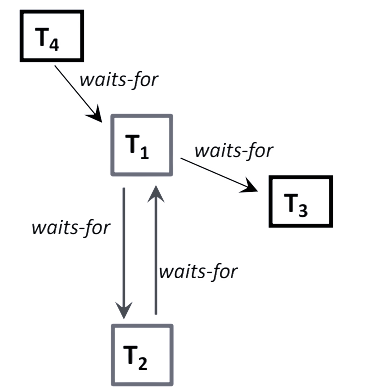
\includegraphics[width=0.35\linewidth]{images/waitgraph.png}
        \caption{An example of deadlock in the wait-for graph}
    \end{figure}
    It is possible to solve deadlocks in three different ways: 
    \begin{itemize}
        \item Timeout: a transaction is killed and restarted after a given amount of waiting, to be determined by the system manager. 
        \item Deadlock prevention: kills transactions that could cause cycles. It is implemented in two ways: 
            \begin{enumerate}
                \item Resource-based prevention puts restrictions on lock requests. The idea is that every transaction requests all resources at once, and only once. The main problem
                    is that it's not easy for transactions to anticipate all requests. 
                \item Transaction-based prevention puts restrictions on transactions' IDs. Assigning IDs to transactions incrementally allows to give an age to each one. It is 
                    possible to choose to kill the holding transaction (preemptive) or the requesting one (non-preemptive). The main problem is that the number of killings is too big. 
            \end{enumerate}
        \item Deadlock detection: it can be implemented with various algorithms and used for distributed resources. 
    \end{itemize}
    \begin{definition}
        The \emph{distributed dependency graph} is a wait-for graph where external call nodes represent a sub-transaction activating another sub-transaction at a different node. 
    \end{definition}
    The arrow shows a wait-for relation among local transactions. If one term is an external call, either the source is waited for by a remote transaction or waits for a remote 
    transaction. The Obermarck's algorithm needs the following assumptions: 
    \begin{itemize}
        \item Transactions execute on a single main node. 
        \item Transactions may be decomposed in sub-transactions running on other nodes. 
        \item When a transaction spawns a sub-transaction it suspends work until the latter completes. 
        \item Two wait-for relationships:
            \begin{itemize}
                \item $T_i$ waits for $T_j$ on the same node because $T_i$ needs a datum locked by $T_j$. 
                \item A sub-transaction of $T_i$ waits for another sub-transaction of $T_i$ running on a different node. 
            \end{itemize}
    \end{itemize}
    The goal of this algorithm is to detect a potential deadlock looking only at the local view of a node. Nodes exchange information and update their local graph based on the 
    received information. Node $A$ sends its local info to a node $B$ only if: it contains a transaction $T_i$ that is waited for from another remote transaction and waits for a 
    transaction $T_j$ active on $B$ and $i>j$.
    \begin{example}
        Given the following distributed dependency graph: 
        \begin{figure}[H]
            \centering
            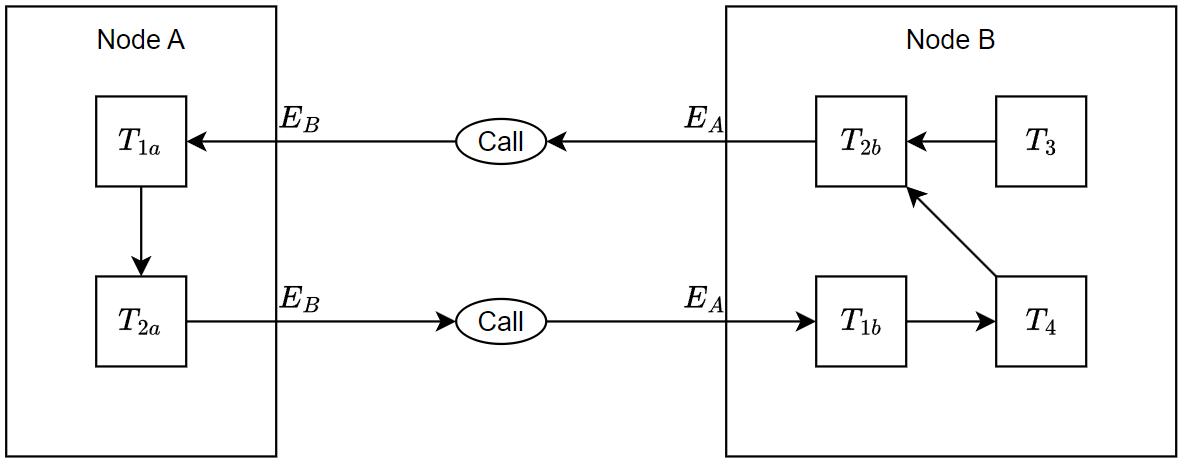
\includegraphics[width=0.5\linewidth]{images/distributedgraph.png}
        \end{figure}
        We can see that the potential deadlock is given by cycles. In this case, we have that $T_{2a}$ waits for $T_{1a}$ (data lock) that waits for $T_{1b}$ (call) that waits for 
        $T_{2b}$ (data locks) that waits for $T_{2a}$ (call). 
        
        In this case the node $A$ dispatches information to $B$, in fact we have $ E_b \rightarrow T_2 \rightarrow T_1 \rightarrow E_b$ and node $B$ cannot dispatch information to 
        $A$, because the forwarding rule is not respected: $E_a \rightarrow T_1 \rightarrow T_2 \rightarrow E_a$. 
    \end{example}
    The Obermarck's algorithm runs periodically at each node and consists in four steps: 
    \begin{enumerate}
        \item Get graph info from the previous nodes.
        \item Update the local graph by merging the received information. 
        \item Check the existence of cycles among transactions denoting potential deadlocks: if found, select one transaction in the cycle and kill it. 
        \item Send updated graph info to the next nodes. 
    \end{enumerate}
    \begin{example}
        Given the following distributed system:
        \begin{figure}[H]
            \centering
            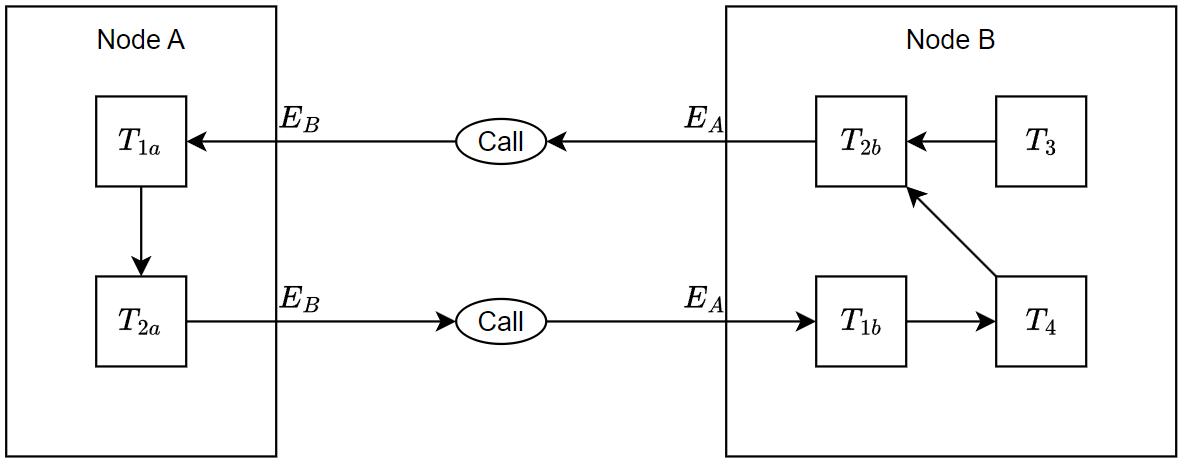
\includegraphics[width=0.5\linewidth]{images/distributedgraph.png}
        \end{figure}
        We want to apply the Obermarck's algorithm: 
        \begin{enumerate}
            \item Use the forwarding rule, in this case we have: 
                \begin{itemize}
                    \item At Node $A$: $E_b \rightarrow T_2 \rightarrow T_1 \rightarrow E_b$ info sent to Node $B$
                    \item At Node $B$: $E_a \rightarrow T_1 \rightarrow T_2 \rightarrow E_a$ info not sent $(i<j)$. 
                \end{itemize}
            \item At node $B$ there is the updated info $E_b \rightarrow T_2 \rightarrow T_1 \rightarrow E_b$ and it is added to the wait-for graph.
            \item At node $B$ a deadlock is detected (cycle between $T_1$ and $T_2$) and $T_1$, $T_2$ or $T_4$ are killed. 
            \item Updated information are sent to all nodes. 
        \end{enumerate}
    \end{example}
    There are four variants of this algorithm, based on various conventions.
    \begin{table}[H]
        \centering
        \begin{tabular}{c|cc|}
        \cline{2-3}
        \textbf{}               & \textbf{Message condition} & \textbf{Message receiver} \\ \hline
        \multicolumn{1}{|l|}{A} & $i>j$                      & Following node            \\
        \multicolumn{1}{|l|}{B} & $i>j$                      & Preceding node            \\
        \multicolumn{1}{|l|}{C} & $i<j$                      & Following node            \\
        \multicolumn{1}{|l|}{D} & $i<j$                      & Preceding node            \\ \hline
        \end{tabular}
    \end{table}
    In practice, the probability of deadlocks ($n^{-2}$) is much less than the conflict probability ($n^{-1}$). There are techniques to limit the frequency of deadlocks: 
    \begin{itemize}
        \item Update lock: the most frequent deadlock occurs when two concurrent transactions start by reading the same resources and then decide to write and try to upgrade their 
        lock to write on the resource. To avoid this situation, systems offer the update lock, that is used by transactions that will read and then write. The lock table become: 
        \begin{table}[H]
            \centering
            \begin{tabular}{ccccc}
            \textbf{}                                     & \multicolumn{4}{c}{\textbf{Resource status}}                                                                                                        \\ \cline{2-5} 
            \multicolumn{1}{c|}{\textbf{Request}}         & \textit{FREE}                     & \textit{SHARED}                   & \textit{UPDATE}                   & \multicolumn{1}{c|}{\textit{EXCLUSIVE}} \\ \hline
            \multicolumn{1}{|c|}{\textit{Shared lock}}    & \multicolumn{1}{c|}{$\checkmark$} & \multicolumn{1}{c|}{$\checkmark$} & \multicolumn{1}{c|}{$\checkmark$} & \multicolumn{1}{c|}{$\tikzxmark$}       \\ \hline
            \multicolumn{1}{|c|}{\textit{Update lock}}    & \multicolumn{1}{c|}{$\checkmark$} & \multicolumn{1}{c|}{$\checkmark$} & \multicolumn{1}{c|}{$\tikzxmark$} & \multicolumn{1}{c|}{$\tikzxmark$}       \\ \hline
            \multicolumn{1}{|c|}{\textit{Exclusive lock}} & \multicolumn{1}{c|}{$\checkmark$} & \multicolumn{1}{c|}{$\tikzxmark$} & \multicolumn{1}{c|}{$\tikzxmark$} & \multicolumn{1}{c|}{$\tikzxmark$}       \\ \hline
            \end{tabular}
        \end{table}
        \item Hierarchical lock: locks can be specified with different granularities. The objective of this is to lock the minimum amount of data and recognize conflicts as soon as
        possible. The method used to do so consists in asking locks on hierarchical resources by requesting resources top-down until the right level is obtained and releasing 
        locks bottom-up. This is done by using five locking modes: shared, exclusive, ISL (intention of locking a sub-element of the current element in shared mode), IXL (intention 
        of locking a sub-element of the current element in exclusive mode), and SIXL (lock of the element in shared mode with intention of locking a sub-element in exclusive mode). 
        The lock table become: 
        \begin{table}[H]
            \centering
            \begin{tabular}{ccccccc}
            \textbf{}                             & \multicolumn{6}{c}{\textbf{Resource status}}                                                                                                                                                                            \\ \cline{2-7} 
            \multicolumn{1}{c|}{\textbf{Request}} & \multicolumn{1}{c|}{\textit{FREE}} & \multicolumn{1}{c|}{\textit{ISL}} & \multicolumn{1}{c|}{\textit{IXL}} & \multicolumn{1}{c|}{\textit{SL}}  & \multicolumn{1}{c|}{\textit{SIXL}} & \multicolumn{1}{c|}{\textit{XL}}  \\ \hline
            \multicolumn{1}{|c|}{\textit{ISL}}    & \multicolumn{1}{c|}{$\checkmark$}  & \multicolumn{1}{c|}{$\checkmark$} & \multicolumn{1}{c|}{$\checkmark$} & \multicolumn{1}{c|}{$\checkmark$} & \multicolumn{1}{c|}{$\checkmark$}  & \multicolumn{1}{c|}{$\tikzxmark$} \\ \hline
            \multicolumn{1}{|c|}{\textit{IXL}}    & \multicolumn{1}{c|}{$\checkmark$}  & \multicolumn{1}{c|}{$\checkmark$} & \multicolumn{1}{c|}{$\checkmark$} & \multicolumn{1}{c|}{$\tikzxmark$} & \multicolumn{1}{c|}{$\tikzxmark$}  & \multicolumn{1}{c|}{$\tikzxmark$} \\ \hline
            \multicolumn{1}{|c|}{\textit{SL}}     & \multicolumn{1}{c|}{$\checkmark$}  & \multicolumn{1}{c|}{$\checkmark$} & \multicolumn{1}{c|}{$\tikzxmark$} & \multicolumn{1}{c|}{$\checkmark$} & \multicolumn{1}{c|}{$\tikzxmark$}  & \multicolumn{1}{c|}{$\tikzxmark$} \\ \hline
            \multicolumn{1}{|c|}{\textit{SIXL}}   & \multicolumn{1}{c|}{$\checkmark$}  & \multicolumn{1}{c|}{$\checkmark$} & \multicolumn{1}{c|}{$\tikzxmark$} & \multicolumn{1}{c|}{$\tikzxmark$} & \multicolumn{1}{c|}{$\tikzxmark$}  & \multicolumn{1}{c|}{$\tikzxmark$} \\ \hline
            \multicolumn{1}{|c|}{\textit{XL}}     & \multicolumn{1}{c|}{$\checkmark$}  & \multicolumn{1}{c|}{$\tikzxmark$} & \multicolumn{1}{c|}{$\tikzxmark$} & \multicolumn{1}{c|}{$\tikzxmark$} & \multicolumn{1}{c|}{$\tikzxmark$}  & \multicolumn{1}{c|}{$\tikzxmark$} \\ \hline
            \end{tabular}
        \end{table}
        \begin{example}
            Given a table $X$ with eight tuples divided in two pages: 
            \begin{table}[H]
                \centering
                \begin{tabular}{cc}
                \textbf{P1}                 & \textbf{P2}               \\ \hline
                \multicolumn{1}{|c|}{$t1$}  & \multicolumn{1}{c|}{$t5$} \\ \hline
                \multicolumn{1}{|c|}{$t2$}  & \multicolumn{1}{c|}{$t6$} \\ \hline
                \multicolumn{1}{|c|}{$t3$}  & \multicolumn{1}{c|}{$t7$} \\ \hline
                \multicolumn{1}{|c|}{$t4$}  & \multicolumn{1}{c|}{$t8$} \\ \hline
                \end{tabular}
            \end{table}
            And two transactions with the following schedules: 
            \[T_1=r(P1)\:w(t3)\:r(t8)\]
            \[T_2=r(t2)\:r(t4)\:w(t5)\:w(t6)\]
            We can see that they are not in a read-write conflict (because they are independent of the order). Without hierarchical locking both transactions needs to operate on the 
            same table, so the concurrency will be almost useless in this case. But with this technique, calling $X$ the table, we have that the transaction acquires the following
            locks: 
            \[T_1:\:IXL(root)\:SIXL(P1)\:XL(t3)\:ISL(P2)\:SL(t8)\]
            \[T_2:\:IXL(root)\:ISL(P1)\:SL(t2)\:SL(t4)\:IXL(P2)\:XL(t5)\:XL(t6)\]
        \end{example}
    \end{itemize}

    \section{Timestamps}
    Locking is also named pessimistic concurrency control because it assumes that collisions will arise. In reality collisions are rare. So, it is possible to use optimistic 
    concurrency control methods like timestamps, which are identifier that defines a total ordering of the events of a system. Each transaction has a timestamp representing the time 
    at which the transaction begins so that transactions can be ordered: the smaller is the index the older is the transaction. A schedule is accepted only if it reflects the serial 
    ordering of the transactions induced by their timestamps. The timestamps are given by a system's function on request. The syntax of a timestamp is the following: 
    \[\textnormal{event-id}.\textnormal{node-id}\]
    The algorithm's synchronization is based on send-receive of messages, and it is called Lamport method. It is based on the following rule: it is not possible to receive a  message 
    from the future, if this happens the bumping rule is used to bump the timestamp of the receive event beyond the timestamp of the send event.     
    \begin{example}
        An example of timestamps assignation at two different nodes can be the following. 
        \begin{figure}[H]
            \centering
            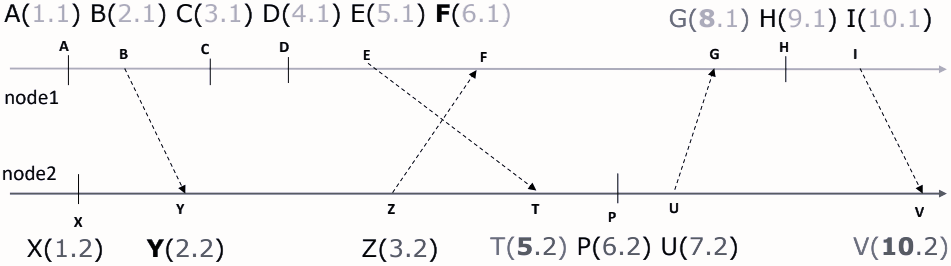
\includegraphics[width=0.75\linewidth]{images/timestamps.png}
        \end{figure}
    \end{example}
    The scheduler uses two counters: one for writes WTM($x$) and another for reads RTM($x$). The scheduler receives read/write requests tagged with the timestamp of the 
    requesting transaction. In case of a read operation we can have: 
    \begin{itemize}
        \item If $ts<\textnormal{WTM}(x)$ the request is rejected and the transaction is killed. 
        \item Else, access is granted, and we set $\textnormal{RTM}(x)=\max(\textnormal{RTM}(x),ts)$. 
    \end{itemize}
    In case of a write operation we can have: 
    \begin{itemize}
        \item If $ts<\textnormal{RTM}(x)$ or $ts<\textnormal{WTM}(x)$ the request is rejected, and the  transaction is killed. 
        \item Else, access is granted, and we set $\textnormal{WTM}(x)=ts$. 
    \end{itemize}
    The problem that arise using this technique is that too many transactions are killed. 
    \begin{example}
        Let us assume $\textnormal{RTM}(x)=7$ and $\textnormal{WTM}(x)=4$ and the following schedule: 
        \[S=r_6(x) r_8(x) r_9(x) w_8(x) w_{11}(x) r_{10}(x)\]
        Using the timestamps we obtain: 
        \begin{table}[H]
            \centering
            \begin{tabular}{ccc}
            \textbf{Request} & \textbf{Response} & \textbf{New value} \\ \hline
            $r_6(x)$         & $\checkmark$      & -                  \\
            $r_8(x)$         & $\checkmark$      & $\textnormal{RTM}(x)=8$         \\
            $r_9(x)$         & $\checkmark$      & $\textnormal{RTM}(x)=9$         \\
            $w_8(x)$         & $\tikzxmark$      & $T_8$ killed       \\
            $w_{11}(x)$      & $\checkmark$      & $\textnormal{WTM}(x)=11$        \\
            $r_{10}(x)$      & $\tikzxmark$      & $T_{10}$ killed   
            \end{tabular}
        \end{table}
    \end{example}
    It is not possible to compare 2PL to TS (this means that there is no subset between the categories). We have only that TS implies CSR. 
    \begin{proof}[TS implies CSR]
        Let $S$ be a TS schedule of $T_1$ and $T_2$. Suppose $S$ is not CSR, which implies that it contains a cycle between $T_1$ and $T_2$. $S$ contains $op_1(x)$, $op_2(x)$ where at 
        least one is a write. $S$ contains also $op_2(y)$, $op_1(y)$ where at least one is a write. 
        When $op_1(y)$ arrives:
        \begin{itemize}
            \item If $op_1(y)$ is a read, $T_1$ is killed by TS because it tries to read a value written by a younger transaction, so it is a contradiction. 
            \item If $op_1(y)$ is a write, $T_1$ is killed no matter what $op_2(y)$ is, because it tries to write a value already read or written by a younger transaction, so it is a 
                contradiction. 
        \end{itemize}
    \end{proof}
    Basic TS-based control considers only committed transactions in the schedule, aborted transactions are not considered. If aborts occur, dirty reads may happen. To cope with dirty 
    reads, a variant of basic TS must be used: a transaction $T_i$ that issues $r_{ts}(x)$ or $w_{ts}(x)$ such that $ts>\textnormal{WTM}(x)$ has its read or write operation delayed until the
    transaction $T^{'}$ that wrote the value of $x$ has committed or aborted. This is similar to long duration write locks, so it introduces delays. 
    \begin{table}[H]
        \centering
        \begin{tabular}{c|cc}
        \textbf{Action} & \textbf{2PL}          & \textbf{TS}          \\ \hline
        Transaction     & Wait                  & Killed and restarted \\
        Serialization   & Imposed by conflicts  & Imposed by timestamp \\
        Delay           & Long (strict version) & Long                 \\
        Deadlocks       & Possible              & Prevented           
        \end{tabular}
    \end{table}
    Since that restarting a transaction is costlier than waiting, 2PL is better if used alone. Commercial system mediates between those techniques to get the better feature from both. 
    To reduce the number of killings it is possible to use the Thomas rule, that changes the rule for the write operations: 
    \begin{itemize}
        \item If $ts<\textnormal{RTM}(x)$ the request is rejected and the transaction is killed. 
        \item Else, if $ts<\textnormal{WTM}(x)$ then our write is obsolete: it can be skipped. 
        \item Else, access is granted, and we set $\textnormal{WTM}(x)=ts$. 
    \end{itemize}

    \section{Multi-version concurrency control}
    The idea of multi-version is that writes generate new versions, and that reads access the right version. Writes generate new copies, each one with a new WTM, so each object $x$ 
    always has $N \geq 1$ active versions. There is a unique global RTM($x$). Old versions are discarded when there are no transactions that need their values. 
    In theory, it is possible to use the following rule: 
    \begin{itemize}
        \item $r_{ts}(x)$ is always accepted. A copy $x_k$ is selected for reading such that:
            \begin{itemize}
                \item If $ts \geq \textnormal{WTM}_N(x)$, then $k=N$.
                \item Else take $k$ such that $\textnormal{WTM}_k(x) \leq ts < \textnormal{WTM}_{k+1}(x)$. 
            \end{itemize}
        \item $w_{ts}(x)$: 
            \begin{itemize}
                \item If $ts < \textnormal{RTM}(x)$ the request is rejected. 
                \item Else a new version is created for timestamp $ts$ ($N$ is incremented). $\textnormal{WTM}_1(x), \dots, \textnormal{WTM}_N(x)$ are the new versions, kept sorted from oldest to youngest.
            \end{itemize}
    \end{itemize}
    \begin{example}
        Let us assume $\textnormal{RTM}(x)=7$, $N=1$ and $\textnormal{WTM}_1(x)=4$ and the following schedule: 
        \[S=r_6(x) r_8(x) r_9(x) w_8(x) w_{11}(x) r_{10}(x) r_{12}(x) w_{14}(x) w_{13}(x)\]
        Using the multi-version we obtain: 
        \begin{table}[H]
            \centering
            \begin{tabular}{ccc}
            \textbf{Request} & \textbf{Response}         & \textbf{New value}  \\ \hline
            $r_6(x)$         & $\checkmark$              & -                   \\
            $r_8(x)$         & $\checkmark$              & $\textnormal{RTM}(x)=8$          \\
            $r_9(x)$         & $\checkmark$              & $\textnormal{RTM}(x)=9$          \\
            $w_8(x)$         & $\tikzxmark$              & $T_8$ killed        \\
            $w_{11}(x)$      & $\checkmark$              & $\textnormal{WTM}_2(x)=11,\:N=2$ \\
            $r_{10}(x)$      & $\checkmark$ on $x_{(1)}$ & $\textnormal{RTM}(x)=10$         \\
            $r_{12}(x)$      & $\checkmark$ on $x_{(2)}$ & $\textnormal{RTM}(x)=12$         \\
            $w_{14}(x)$      & $\checkmark$              & $\textnormal{WTM}_3(x)=14,\:N=3$ \\
            $w_{13}(x)$      & $\checkmark$              & $\textnormal{WTM}_4(x)=14,\:N=4$
            \end{tabular}
        \end{table}
    \end{example}

    In practice, it is possible to use the following rule: 
    \begin{itemize}
        \item $r_{ts}(x)$ is always accepted. A copy $x_k$ is selected for reading such that:
            \begin{itemize}
                \item If $ts \geq \textnormal{WTM}_N(x)$, then $k=N$. 
                \item Else take $k$ such that $\textnormal{WTM}_k(x) \leq ts < \textnormal{WTM}_{k+1}(x)$. 
            \end{itemize}
        \item $w_{ts}(x)$:
            \begin{itemize}
                \item If $ts < \textnormal{RTM}(x)$ or $ts < \textnormal{WTM}_N(x)$ the request is rejected. 
                \item Else a new version is created for timestamp $ts$ ($N$ is incremented)
                \item $\textnormal{WTM}_1(x), \dots, \textnormal{WTM}_N(x)$ are the new versions, kept sorted from oldest to youngest. 
            \end{itemize}
    \end{itemize}
    \begin{example}
        Let us assume $\textnormal{RTM}(x)=7$, $N=1$ and $\textnormal{WTM}_1(x)=4$ and the following schedule: 
        \[S=r_6(x) r_8(x) r_9(x) w_8(x) w_{11}(x) r_{10}(x) r_{12}(x) w_{14}(x) w_{13}(x)\]
        Using the multi-version we obtain: 
        \begin{table}[H]
            \centering
            \begin{tabular}{ccc}
            \textbf{Request} & \textbf{Response}         & \textbf{New value}  \\ \hline
            $r_6(x)$         & $\checkmark$              & -                   \\
            $r_8(x)$         & $\checkmark$              & $\textnormal{RTM}(x)=8$          \\
            $r_9(x)$         & $\checkmark$              & $\textnormal{RTM}(x)=9$          \\
            $w_8(x)$         & $\tikzxmark$              & $T_8$ killed        \\
            $w_{11}(x)$      & $\checkmark$              & $\textnormal{WTM}_2(x)=11,\:N=2$ \\
            $r_{10}(x)$      & $\checkmark$ on $x_{(1)}$ & $\textnormal{RTM}(x)=10$         \\
            $r_{12}(x)$      & $\checkmark$ on $x_{(2)}$ & $\textnormal{RTM}(x)=12$         \\
            $w_{14}(x)$      & $\checkmark$              & $\textnormal{WTM}_3(x)=14,\:N=3$ \\
            $w_{13}(x)$      & $\tikzxmark$              & $T_{13}$ killed
            \end{tabular}
        \end{table}
    \end{example}
    The final structure for the sets is the following. 
    \begin{figure}[H]
        \centering
        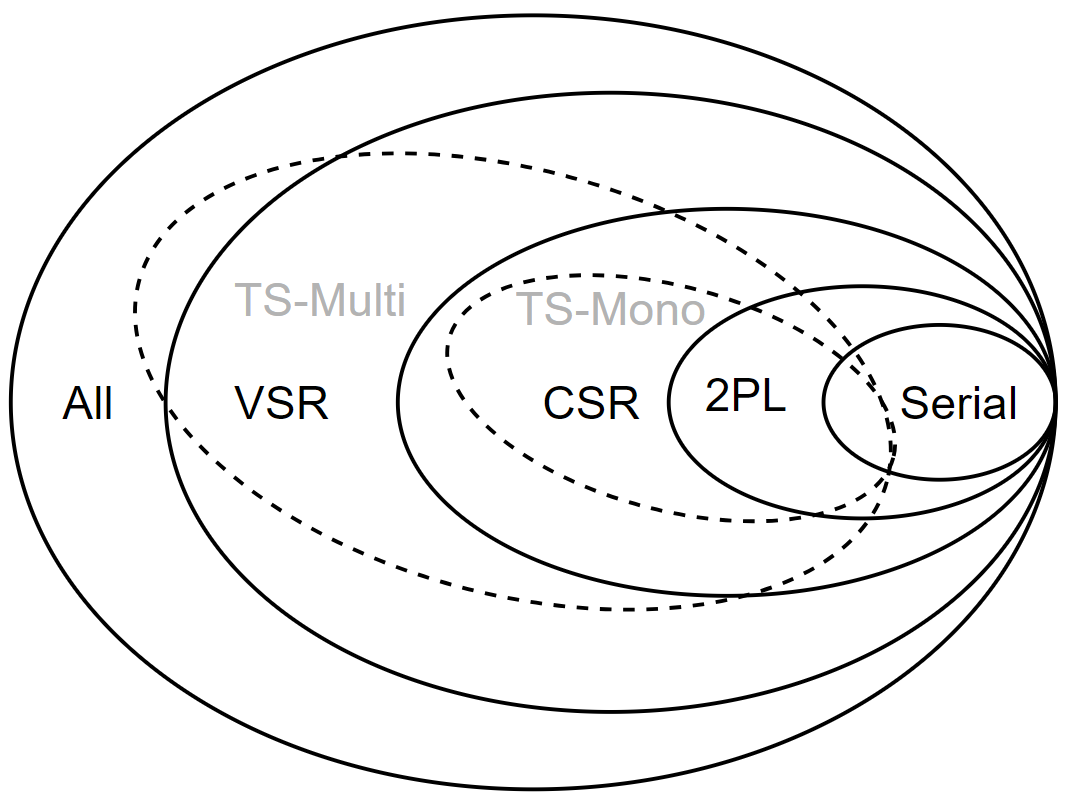
\includegraphics[width=0.75\linewidth]{images/set.png}
        \caption{Set structure for concurrency classification}
    \end{figure}
    The realization of TS-Multi gives the opportunity to introduce into the DBMS another isolation level called snapshot isolation. In this level only WTM($x$) is used. The rule 
    used in this level states that every transaction reads the version consistent with its timestamp, and defers writes to the end. If the scheduler detects that the writes of a
    transaction conflict with writes of other concurrent transactions after the snapshot timestamp, it aborts. Snapshot isolation does not guarantee serializability: it is possible 
    to have a new anomaly called write skew (the order of the operation can change in different executions changing the final result). 
    
\newpage 

\chapter{Ranking}
    \section{Introduction}
    Data are: available in large quantities, represented under many models, queried with many languages, and processed with many algorithms. We can use ranking to get the best
    result out of the data. To do this we have to use the so called multi-objective optimization, that consist in the simultaneous optimization of different criteria. A general 
    multi-objective problem can be formulated as follows: given $N$ objects described by $d$ attributes, we need to find the best $k$ objects. 
    
    This problem is relevant in many fields, for instance: search engines, e-commerce, recommender systems, and Machine Learning. 

    The main approaches to solve the multi-objective optimization are: 
    \begin{itemize}
        \item Ranking queries: selects the top $k$ objects according to a given scoring function.
        \item Skyline queries: selects the set of non-dominated objects. 
    \end{itemize}

    \section{History}
    Rank aggregation is the problem of combining several ranked lists of objects in a robust way to produce a single consensus ranking of the objects. 

    In the $13^{\textnormal{th}}$ century started this problem was introduced with the elections polls. Borda proposed to give a number of penalty points equivalent to the position 
    of the electors in a voter's ranking, so the winner will be the candidate with the lowest overall penalty. Condorcet, instead, proposed to consider as winner the candidate who 
    defeats every other candidate in pairwise majority rule election. The winner with two methods can be different. 
    \begin{example}
        Given ten voters and three candidates with the following votes: 
        \begin{table}[H]
            \centering
            \begin{tabular}{|c|c|c|c|c|c|c|c|c|c|}
            \hline
            1 & 2 & 3 & 4 & 5 & 6 & 7 & 8 & 9 & 10 \\ \hline
            A & A & A & A & A & A & C & C & C & C  \\ 
            C & C & C & C & C & C & B & B & B & B  \\ 
            B & B & B & B & B & B & A & A & A & A  \\ \hline
            \end{tabular}
        \end{table}
        For Borda we have: 
        \begin{itemize}
            \item $A: 1 \cdot 6+3 \cdot 4 = 18$
            \item $B: 3 \cdot 6+2 \cdot 4 = 26$
            \item $C: 2 \cdot 6+1 \cdot 4 = 16$ (winner)
        \end{itemize}
        While for Condorcet we have that $A$ beats both $B$ and $C$ in pairwise majority, so it is the winner. So, the winner is different and depends on the method used. 
    \end{example}

    In 1950 Arrow proposed the axiomatic approach. He defined the aggregation as axioms and understood that a small set of natural requirements cannot be simultaneously achieved by 
    any nontrivial aggregation function. So, he stated the Arrow's paradox: no rank-order electoral system can be designed that always satisfies these fairness criteria:
    \begin{itemize}
        \item No dictatorship (nobody determines, alone, the group's preference). 
        \item If all prefer $X$ to $Y$, then the group prefers $X$ to $Y$. 
        \item If, for all voters, the preference between $X$ and $Y$ is unchanged, then the group preference between $X$ and $Y$ is unchanged. 
    \end{itemize}

    To solve this paradox, in the later years researchers tried to measure the values of all analyzed objects and created the metric approach. This consist in finding a new ranking 
    $R$ whose total distance to the initial rankings $R_1,\dots,R_n$ is minimized. The distance between rankings can be found in several ways: 
    \begin{itemize}
        \item Kendall tau distance $K(R_1, R_2)$, defined as the number of exchanges in a bubble sort to convert $R_1$ to $R_2$. 
        \item Spearman's foot-rule distance $F(R_1, R_2)$, which adds up the distance between the ranks of the same item in the two rankings. 
    \end{itemize}
    Finding an exact solution is computationally hard for Kendall tau (NP-complete), but tractable for Spearman's foot-rule (P time). These distances are related:
    \[K(R_1, R_2) \leq F(R_1, R_2) \leq 2K(R_1, R_2)\]
    And it is possible to find efficient approximation for $F(R_1, R_2)$. 

    \section{Opaque rankings}
    The technique that works on opaque rankings are those which use only the position of the elements in the ranking and no other associated score. The algorithm called MedRank is
    based on the notion of median and provides an approximation of the Foot-rule optimal aggregation. The inputs of this algorithm are: an integer $k$ and a ranked list 
    $R_1,\dots,R_m$ of $N$ elements. The output is the top k elements according to median ranking. The idea of the algorithm is the following: 
    \begin{enumerate}
        \item Use sorted accesses in each list, one element at a time, until there are $k$ elements that occur in more than $m/2$ lists.
        \item These are the top $k$ elements. 
    \end{enumerate}
    \begin{definition}
        The maximum number of sorted accesses made on each list is also called the \emph{depth reached} by the algorithm. 
    \end{definition}
    \begin{example}
        Suppose we have to sort the hotels based on three rankings criteria: price, rating, and distance. Using the MedRank algorithm we can make e one sorted access at a time in 
        each ranking and then look for hotels that appear in at least two rankings. We assume that price, rating and distance are opaque, so only the rank's position matters. The 
        ranks of hotels are the following:
        \begin{table}[H]
            \centering
            \begin{tabular}{c|c|c}
            \textbf{Price} & \textbf{Rating} & \textbf{Distance} \\ \hline
            Ibis           & Crillon         & Le Roch           \\
            Etap           & Novotel         & Lodge In          \\
            Novotel        & Sheraton        & Ritz              \\
            Mercure        & Hilton          & Lutetia           \\
            Hilton         & Ibis            & Novotel           \\
            Sheraton       & Ritz            & Sheraton          \\
            Crillon        & Lutetia         & Mercure           \\
            $\dots$        & $\dots$         & $\dots$          
            \end{tabular}
        \end{table}
        If we use MedRank with $k=3$, we will obtain the following rank: 
        \begin{table}[H]
            \centering
            \begin{tabular}{cc}
            \hline
            \textbf{Top k hotels}       & \textbf{Median rank}          \\ \hline
            Novotel                     & median$\{2,3,5\}=3$           \\ 
            Hilton                      & median$\{4,5,?\}=5$           \\ 
            Ibis                        & median$\{1,5,?\}=5$           \\ \hline
            \end{tabular}
        \end{table}
        The depth in this case is equal to five. 
    \end{example}
    \begin{definition}
        An algorithm is \emph{optimal} if its execution cost is never worse than any other algorithm on any input.
    \end{definition}
    MedRank is not optimal, but it is instance optimal. This means that among the algorithms that access the lists in sorted order, this is the best possible algorithm on every 
    input instance. In other words, its cost cannot be arbitrarily worse than any other algorithm on any problem instance. The instance optimality is a form of optimality aimed 
    at when standard optimality is unachievable. 
    \begin{definition}
        Let $\textbf{A}$ be a family of algorithms, $\textbf{I}$ a set of problem instances. Let cost be a cost metric applied to an algorithm-instance pair. Algorithm 
        $A^{*}$ is instance-optimal with respect to $\textbf{A}$ and $\textbf{I}$ for the cost metric cost if there exist constants $k_1$ and $k_2$ such that, for all 
        $A \in \textbf{A}$ and $I \in \textbf{I}$: 
        \[\textnormal{cost}(A^{*}, I) \leq k_1 \textnormal{cost}(A, I) + k_2\]
    \end{definition}
    If $A^{*}$ is instance-optimal, then any algorithm can improve with respect to $A^{*}$ by only a constant factor $r$, which is therefore called the optimality ratio of $A^{*}$. 
    Instance optimality is a much stronger notion than optimality in the average or worst case. 

    \section{Ranking queries}
    Ranking queries, also called top-$k$ queries, aim to retrieve only the $k$ best answers from a potentially very large result set. Ranking is based on ordering objects based on their relevance.

    Assume a scoring function $S$ that assigns to each tuple $t$ a numerical score for ranking tuples. The algorithm needs this inputs: cardinality $k$, dataset $R$, scoring function $S$. The output is 
    the $k$ highest-scored tuples with respect to $S$. The idea is the following: 
    \begin{enumerate}
        \item For all tuples $t$ in $R$ compute $S(t)$. 
        \item Sort tuples based on their scores.
        \item Return the first $k$ highest-scored tuples. 
    \end{enumerate}
    This naïve approach is expensive for large dataset because it requires to sort a large amount of data. It is even worse if more than one relation is involved because it needs to join all tuples. So, 
    we now know that two abilities are required: 
    \begin{itemize}
        \item Ordering the tuples according to their scores. This is taken care of by 
            \begin{lstlisting}[language=SQL]
ORDER BY
            \end{lstlisting}
        \item Limiting the output cardinality to $k$ tuples. This is taken care (since 2008) of by 
            \begin{lstlisting}[language=SQL]
FETCH FIRST k ROWS ONLY
            \end{lstlisting}
    \end{itemize} 
    \begin{example}
        Consider the following queries: 
        \begin{lstlisting}[language=SQL]
a)  SELECT *
    FROM UsedCarsTable
    WHERE Vehicle = 'Audi/A4'
    AND Price <= 21000
    ORDER BY 0.8*Price+0.2*Miles
b)  SELECT *
    FROM UsedCarsTable
    WHERE Vehicle = 'Audi/A4'
    ORDER BY 0.8*Price+0.2*Miles
        \end{lstlisting}
        The values 0.8 and 0.2, also called weights, are a way to normalize our preferences on price and mileage.
        Query a will likely miss some relevant answers (near-miss). Query b will return all Audi/A4 in the dataset (information overload).
    \end{example}
    Only the first $k$ tuples become part of the result. If more than one set of $k$ tuples satisfies the ordering directive, any of such sets is a valid answer 
    (non-deterministic semantics). 
\end{document}